\chapter{The SEXTANTE toolbox}

\section {Introduction}

The \emph{Toolbox} is the main element of the SEXTANTE GUI, and the one that you are more likely to use in your daily work. It shows the list of all available algorithms grouped in different blocks, and is the access point to run them whether as a single process or as a batch process involving several executions of a same algorithm on different sets of inputs.

\begin{center}
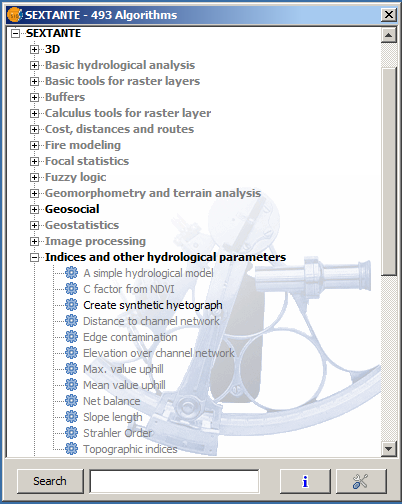
\includegraphics[width=.5\columnwidth]{toolbox.png}
\end{center}

Depending on the data available in the GIS, you will be able to execute an algorithm or not. When there is enough data for the algorithm to be executed (i.e. the algorithm requires raster layers and you have raster layer already loaded into the GIS), its name is shown in black, otherwise, it is shown in grey.

In the lower part of the toolbox you can find a text box and a search button. To reduce the number of algorithms shown in the toolbox and make it easier to find the one you need, you can enter any word or phrase on the text box and click on the search button. SEXTANTE will search the help files associated to each algorithm and show only those algorithms that include the word or phrase in their corresponding help files. To show all the algorithms again, make a search with an empty string.

Notice that, as you type, the number of algorithms in the toolbox is reduced. A search is performed as you type, but only on the algorithm names, not the hep files. You can use this also to quickly find and algorithm. In case you want to perform a full search and look for a given word not just in the algorithm names but also in their associated help files, click the Search button or hit the Enter key.

The configuration button can be found on the search panel as well. It gives access to a new dialog that you can use to configure SEXTANTE. 

\begin{center}
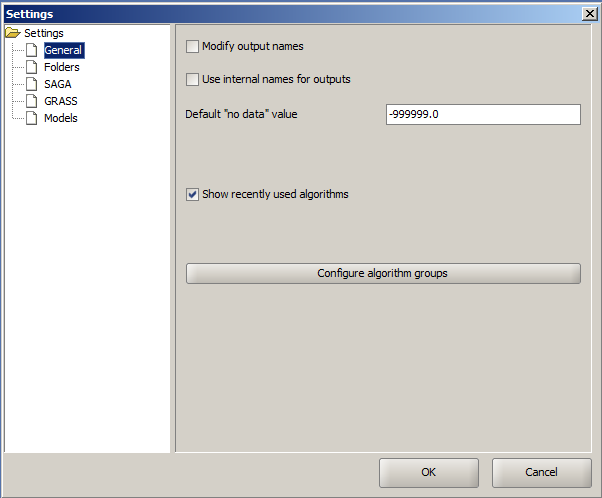
\includegraphics[width=.6\columnwidth]{config_dialog.png}
\end{center}

The meaning of each one of its parameters will be explained in the following pages.

To execute an algorithm, just double--click on its name in the toolbox.

\section{The algorithm dialog}

Once you double--click on the name of the algorithm that you want to execute, a dialog similar to the next one is shown (in this case, the dialog corresponds to the \emph{Anisotropic cost} algorithm).

\begin{center}
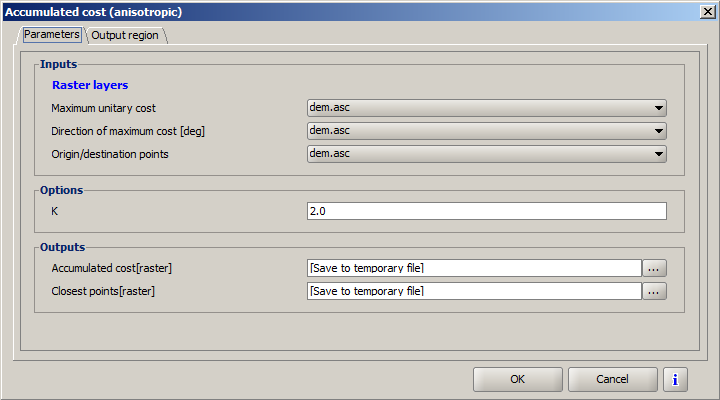
\includegraphics[width=.8\columnwidth]{accumulated_cost_anisotropic.png}
\end{center}

This dialog is used to set the input values that the algorithm needs to be executed.

There is a main tab named \emph{Parameters} where input values and configuration parameters are set. This tab has a different content depending on the requirements of the algorithm to be executed, and is created automatically based on those requirements. On the left side, the name of the parameter is shown. On the right side the value of the parameter can be set.

Most algorithms have an additional tab named \emph{Output extent}. This tab is used to define the region that wants to be analyzed, in case you do not want to perform analysis on the whole extent defined by the input layers.  Also, it should be used to set the characteristics of output raster layers, specifying its extent and its cell size.

On the lower part of the window there is a help button. Click on it to see the context help related to the current algorithm, where you will find detailed description of each parameter and each output generated by the algorithm.

\subsection{The parameters tab}

Although the number and type of parameters depends on the characteristics of the algorithm, the structure is similar for all of them. The parameters found on the parameters tab can be of one of the following types.

\begin{itemize}
	\item A raster layer, to select from a list of all the ones available in the GIS application
	\item A vector layer, to select from a list of all the ones available in the GIS application
	\item A table, to select from a list of all the ones available in the GIS application
	\item A method, to choose from a selection list of possible options
	\item A numerical value, to be introduced in a text box. 
	\item A text string, to be introduced in a text box
	\item A field, to choose from the attributes table of a vector layer or a single table selected in another parameter.
	\item A band, to select from the ones of a raster layer selected in another parameter. In both this and the previous type of parameter, the list of possible choices depends on the value selected in the parent parameter.
	\item A list of elements (whether raster layers, vector ones or tables), to select from the list of the ones available in the GIS application. To make the selection, click on the small button on the left side of the corresponding row to see a dialog like the following one.
		\begin{center}
		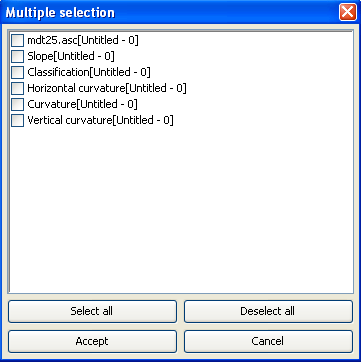
\includegraphics[width=.4\columnwidth]{multiple_selection.png}
		\end{center}
	\item A file or folder
	\item A point, to be introduced as a pair of coordinates in two text boxes (X and Y coordinates). Alternatively, you can click on the button on the right side and select one of the points captured using the \emph{Coordinate Capture} tool (you will find it along with the other SEXTANTE tools. Just select it and click on a view or map in your GIS, and it will get the coordinates of the point where you have clicked). 

	\item A small table to be edited by the user. These are used to define parameters like lookup tables or convolution kernels, among others.

	Click on the button on the right side to see the table and edit its values. 
\begin{center}
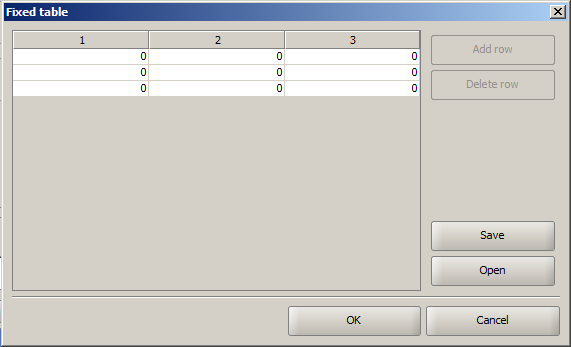
\includegraphics[width=.8\columnwidth]{fixed_table.png}
\end{center}

Depending on the algorithm, the number of rows can be modified or not, using the buttons on the right side of the window.

\end{itemize}

If you have previously executed an algorithm (whether in this work session or in another one), you will find an additional component in the lower left part of the parameters tab.

\begin{center}
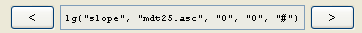
\includegraphics[width=.8\columnwidth]{previous_parameters.png}
\end{center}

By default, in this the parameters are set to the values they had in the last execution. Using the arrow buttons you can change to the values used in previous executions, browsing the SEXTANTE history.

\subsection{The analysis region tab}

The \emph{Analysis region} tab is found in those algorithms in which the user can select the extent of the region to be used for analysis. In most cases, this extent is also used to generate new layers. This is particularly important in the case of raster layers, and in that case not only the extent is needed, but also a value for the cellsize.

Unlike in most GIS, when combining several raster layers as input for an algorithm, they do not have to have the same extent and cellsize in order to process them together. That is, layers don't have necessarily to ``match'' between them. Instead, the characteristics of the analysis region (which are the ones used for the resulting raster layers, in case the algorithm generates such an output) are defined and SEXTANTE performs the corresponding resampling and cropping needed to generate layer with those characteristics. 

It is responsibility of the user to enter adequate values and be aware of the limitations of this mechanism, so as to generate cartographically sound results. (i.e. you can select a small cell size for the resulting raster layers, but if the input layers you are using have a coarse resolution the results will not be geographically sound).

The following options are available in the \emph{Analysis region} tab:

\begin{itemize}

	\item Fit to input layers. By default, the extent is set based on the input layers. The minimum extent needed to cover all the input layers is used.

\begin{center}
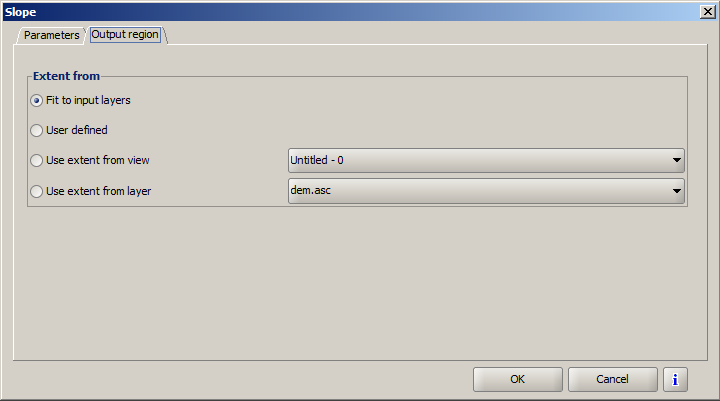
\includegraphics[width=.7\columnwidth]{fit_to_input_layers.png}
\end{center}

	\item User defined. The coordinates of the boundaries of the extent and the cellsize are both defined manually, entering the desired values in the corresponding text boxes. You will be prompted to enter a cellsize always, no matter if the algorithm is just a vector one. Just ignore it and leave the default value, since the algorithm will not use it.
	
\begin{center}
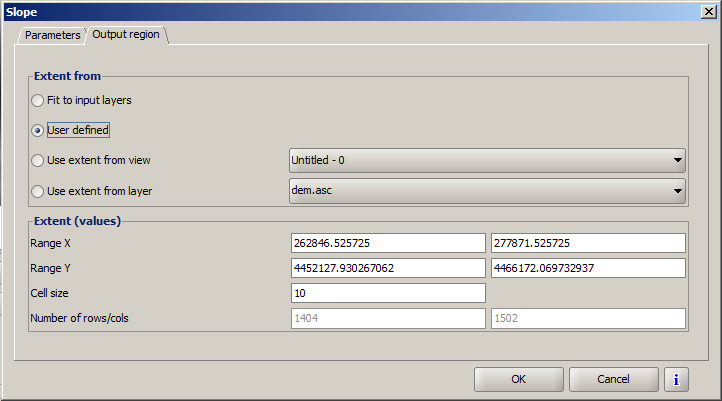
\includegraphics[width=.7\columnwidth]{user_defined.png}
\end{center}

	\item Use predefined extent. Depending on the GIS you are using, this option will let you use predefined extents like, for instance, the extent of one of the views currently opened.
	
\begin{center}
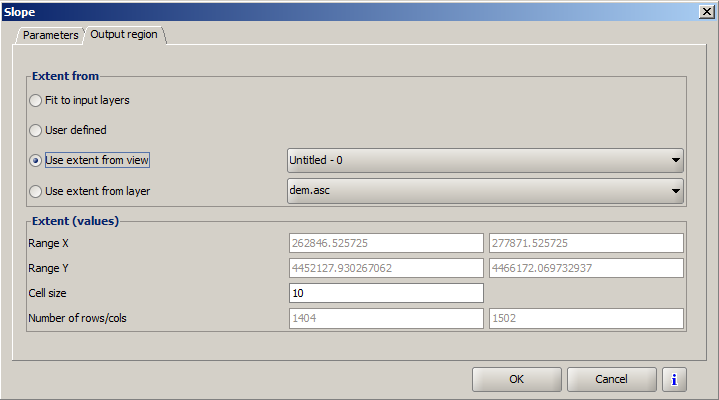
\includegraphics[width=.7\columnwidth]{extent_from_view.png}
\end{center}
	
	
	\item Use extent from layer. The extent of a layer can be used as well to define the analysis region, even if the layer is not used as input to the algorithm. If the selected layer is a vector one, the cellsize will have to be entered manually, since vector layers do not have an associated cellsize.

\begin{center}
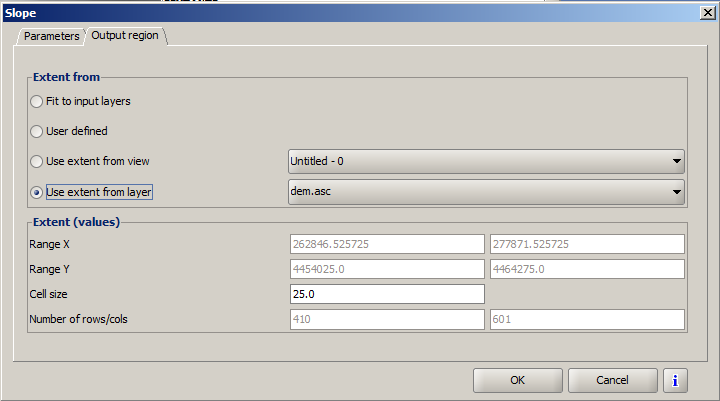
\includegraphics[width=.7\columnwidth]{extent_from_layer.png}
\end{center}

\end{itemize}

If an option other than the automatic fitting is selected, SEXTANTE will check that the values are correct and the resulting raster layers will not be too large (due to, for instance, a wrong cell size). If the output layers seems to large, SEXTANTE will show the next message dialog to ensure that the user really wants those layers to be created.

\begin{center}
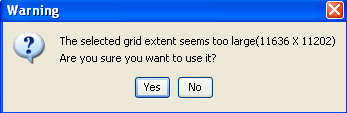
\includegraphics[width=.4\columnwidth]{warning.png}
\end{center}

Not all algorithms have the first option available, since not all algorithms that generate layers take some other similar layer as input. The interpolation algorithms, for instance, take a vector layer and create a raster one. The extent and cellsize of the latter has to be manually defined, since it cannot be set based solely on the input vector layer (vector layers do not have a cellsize value).

\section{Data objects generated by SEXTANTE algorithms}

Data objects generated by SEXTANTE can be of any of the following types:

\begin{itemize}
 \item A raster layer
\item A vector layer
\item A table
\item A graphical result (chart, graph, etc.)
\item A text--only HTML--formatted result
\end{itemize}

Layers and tables can be saved, and the parameters window will contain a text box corresponding to each one of these outputs, where you can type the output channel to use for saving it. An output channel contains the information needed to save the resulting object somewhere. In the most usual case, you will save it to a file, but the architecture of SEXTANTE allows for any other way of storing it. For instance, a vector layer can be stored in a database or even uploaded to a remote server using a WFS--T service. Although solutions like these are not yet implemented, SEXTANTE can now easily handle them, and we expect to add new kinds of output channels in a near feature.



%\begin{center}
%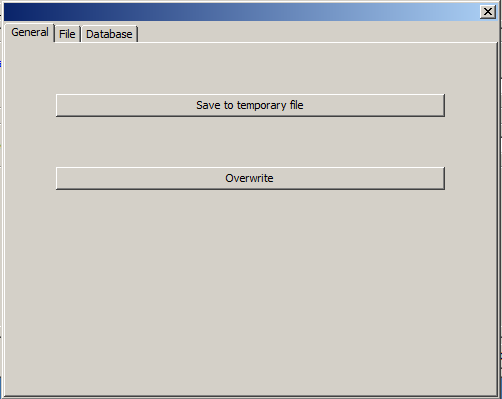
\includegraphics[width=.7\columnwidth]{output_channels.png}
%\end{center}

To select an output channel, just click on the button on the right side of the text box. You will see a dialog with several tabs, each of them containing the elements needed to define a certain kind of output channel. Just go to the tab representing the one that you want and enter the information required. For instance, the File tab is just a file chooser where you have to select a file or type its name. When you are done, click on the OK button.

The first tab you see contains two general options, with a button for each one:

\begin{itemize}
	\item Save to temporary file
	\item Do not create this output
\end{itemize}

Clicking on the ``Save to temporary file'' button will cause SEXTANTE to select a temporary file for saving the resulting data object. That file will be deleted once you exit the GIS and SEXTANTE is shut down. This options should be used when you are executing an algorithm and want to use its results as intermediate data, but do not want to keep them permanently.

Clicking on the ``Do not create this outut'' output will cause the output to be generated, but not stored anywhere and not added to your GIS. This is useful if the algorithm you are running generates several ouputs but you are not interested in all of them.

An ``Overwrite'' option will appear in those algorithms that allow overwriting of input layers. In that case, the algorithm will replace the data of an input layer (the algorithm itself has to \emph{know} which layer from all the input ones) instead of generating a new one. A warning might be shown if the input layer cannot be overwritten (such as, for instance, a layer on a database that the user has no rights to edit). This option is  currently only available for vector layers, and just in some algorithms were it makes sense.

Since file outputs are the most common ones, we will give some extra information about them.

The format of the output is defined by the filename extension. The supported formats depend on the ones supported by the GIS onto which SEXTANTE is running. That means that SEXTANTE usually supports all the formats that the GIS is capable of writing. To select a format, just select the corresponding file extension. If the extension of the filepath you entered does not match any of the supported ones, a default extension (usually dbf for tables, tif for raster layers and shp for vector ones) will be appended to the filepath and the file format corresponding to that extension will be used to save the layer or table.

You can set a default folder for output data objects. Go to the configuration dialog (you can open it from the toolbox), and in the ``Folders'' tab you will find a text box named ``Output folder''. This output folder is used as the default path in case you type just a filename with no path (i.e. \texttt{myfile.shp}) when executing an algorithm. 

Sometimes, layers might have names that include special characters. For example, if you rasterize a layer named ``mylayer'', the result will be a new layer named ``mylayer[rasterized]''. Those brackets can cause you some problems if you later want to use that layer as input for the raster calculator, or from the command--line interface, so it can be a good idea to remove them (the same happens with other characters such as ``�'' or ``�'' that might appear if you use SEXTANTE in spanish). You can tell SEXTANTE to automatically replace those character with valid standard ones. To do so, open the configuration dialog and select the ``General'' group. Select the check box with the label ``Modify output names''.

Apart from raster layers and tables, SEXTANTE also generates graphics and texts. These results are kept in memory and shown at the end of the algorithm execution in a new dialog. This dialog will keep the results produced by SEXTANTE during the current session, and can be shown at any time using the \emph{Results} button.

You can save graphical results as images in png format, and texts as HTML files. Right--click on the name of the result in the tree on the left hand of the window and select \emph{Save as...}.


\begin{center}
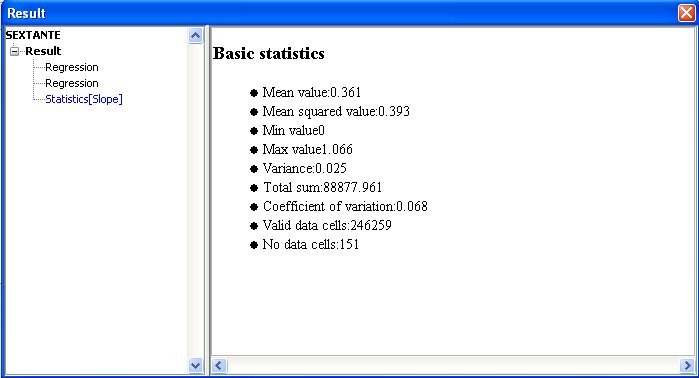
\includegraphics[width=.7\columnwidth]{information_square.png}
\end{center}
 
\begin{center}
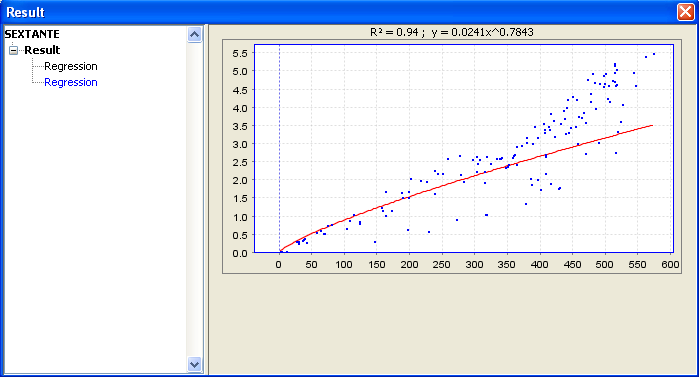
\includegraphics[width=.7\columnwidth]{graphic.png}
\end{center}


\section{Context help}

Each SEXTANTE algorithm has its own context help file, which provides detailed information about the meaning of each input parameter and each output object, and gives hints about its usage. To access the context help system, click on the button that you will find in the algorithm dialog, or right--click on its name on the toolbox and then select \emph{Show help}.

\begin{center}

\includegraphics[width=.8\columnwidth]{help.png}
\end{center}

The context help system contains not only information about each algorithm, but also descriptions of each one of the elements of the SEXTANTE GUI like the text you are reading now. You will find a help button in each element, which will take you to the corresponding help file.


Selecting the \emph{Show help} option from the toolbar, you can access the whole SEXTANTE context help. You will see a window like the one shown next.


		\begin{center}
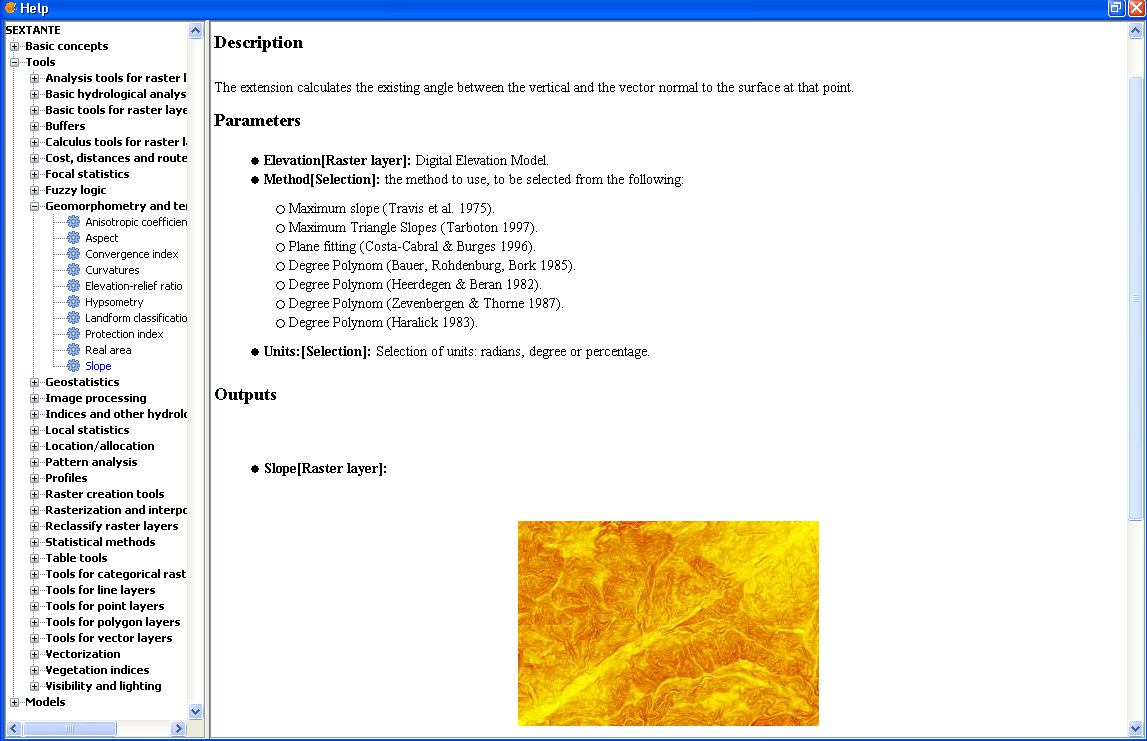
\includegraphics[width=.9\columnwidth]{help_slope.png}
\end{center}

Just click on the topic you want to read on the left--hand side of the window, and its corresponding text will be shown in the right--hand side.

Help files associated to SEXTANTE algorithms are stored as XML files, and can be edited using the help authoring tools included with SEXTANTE. Right click on the name of the algorithm in the context help window and select \emph{Edit help} to get to the following window:


\begin{center}
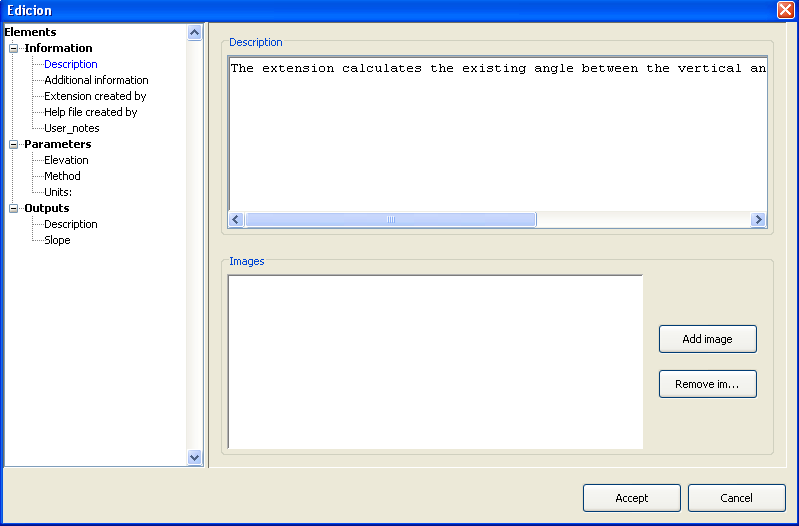
\includegraphics[width=.8\columnwidth]{help_edition.png}
\end{center}

On the left--hand side you can select any of the elements to be documented (input parameter and outputs, along with other fixed field such as a general description of the algorithm). Then use the right--hand side boxes to enter the text associated to that element or add images.

\section{Configuring SEXTANTE}

As we have seen, the configuration button in the lower part of the toolbox gives access to a new dialog where you can configure how SEXTANTE works. Configuration parameters are structured in separate blocks that you can select on the left--hand side of the dialog.

\subsection{General}

You will see two check boxes in the upper part of this group:

\begin{itemize}
 \item \textbf{Modify output names}: if you check this option, output names will be modified to avoid characters such as brackets, blank spaces or stress marks.
  \item  \textbf{Use internal names for outputs}: when this option is selected, SEXTANTE uses internal names to name output layers. This is useful if you plan to use the command--line interface to write scripts, since the names of the outputs can be know in advance (having a look at the help files, under the \emph{Command--line usage} will inform you of those names). If this options is not selected, SEXTANTE will produce layers with names that depend on the current language or sometimes on the names of the input layers, which can cause you trouble if you plan to use those layers for your script.
\end{itemize}

Under that, you will two elements to configure the list of algorithms in the toolbox. The first one can be used to remove the \emph{Most recently used} group in the toolbox. Just uncheck the check box and you will not see that group.

The second one is a button that can be used to redefine how algorithms are organized in the toolbox. Click on the button to get to the following dialog.

\begin{center}
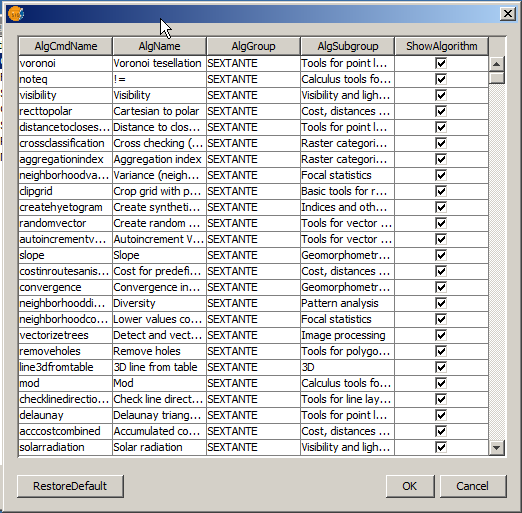
\includegraphics[width=.65\columnwidth]{config_groups.png}
\end{center}

In it, you can change the group and subgroup each algorithm belongs to, and also you can select whether to show or not a given algorithm. Type on the table cells to enter an alternative group of subgroup for an algorithm. Once you are done, click on the OK button. You can restore the default groupings by clicking on the ''Restore default�� button.

\subsection{Folders}

One folder can be defined:

\begin{itemize}
 \item \textbf{Output folder}: when entering the filename for an output layer, if it does not include a valid path, it will be saved to this default output folder.
 \end{itemize}
 
\subsection{Model}

The folder where models are stored has to be set in this field. This will be explained in detail in the following chapter. Once you have entered the path to the folder that you want to use, click on the button below to make SEXTANTE load all the models found there.


\subsection{GRASS, SAGA and other additional algorithm providers}

The set of algorithms of SEXTANTE can be extended by using additional algorithm providers that wrap algorithms from a third--party software. SEXTANTE acts as a front--end to those applications and can reuse their algorithms. Configuration of algorithm providers depends on the characteristics of the provider itself and the software being called from SEXTANTE. This is explained in detail in a separate chapter at the end of this manual.


\section{Iterative execution of algorithms}

SEXTANTE algorithms can be executed iteratively when they include some kind of vector input. In this case, for a layer containing $n$ features, the algorithm is executed $n$ times, each time taking an input layer that contains just one feature from the original layer.

This is useful for certain processes, like, for instance, cropping a raster layer using a vector layer with polygons. Given a polygon layer, the raster layer can be cropped in smaller ones, each of them covering the minimum extent needed to include each one of the input polygons. This will require executing the corresponding algorithm as many times as polygons are contained in the vector layer, which might be a long and tedious process. Instead, executing the algorithm iteratively will automate the task, solving the problem in just one single step.

To execute an algorithm iteratively, right click on its name in the toolbox. You will see a new menu named \emph{Execute iteratively [parameter name]}. There will be as many menus as vector layers the algorithm takes. You can only iterate over one of them, so you have to select the right one depending on what you want to do.

Clicking on the chosen menu, the usual algorithm dialog is shown. It is exactly like the dialog you would see if executing the algorithm the usual way. Just fill in the parameter values and click on \emph{OK}. The progress dialog will inform you of the step that is currently being executed. Resulting layers will be added to the GIS GUI as usual.

When executing iteratively an algorithm that produces text output with numerical values (such as, for instance, statistics of a raster layer), it might be convenient to present those results in a different manner. Otherwise, combining a large number of such text outputs would be difficult and not practical. For this reason, when an algorithms is executed iteratively, its numerical outputs (in case the algorithm generates them) are presented in a table in the results manager. Each row of the table represents an execution of the algorithm, while each column contains the values of one of the numerical variables being calculated.

The following picture shows an example of one of such tables.

\begin{center}
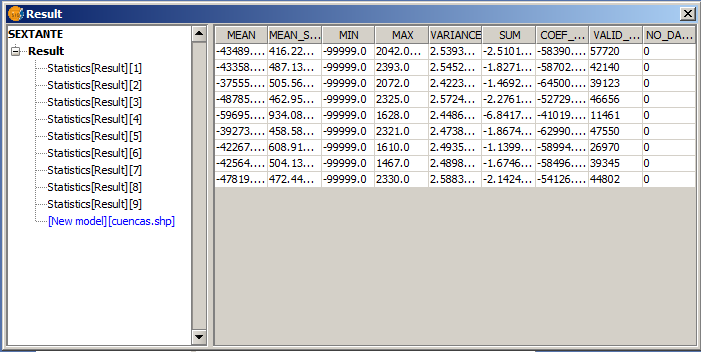
\includegraphics[width=.85\columnwidth]{numerical_table.png}
\end{center}